
\chapter{Polyhedra}\label{chap1}

\section{Definition of Polyhedra}\label{chap1-sec1.1}

Basic units\pageoriginale out of which polyhedra can be constructed are convex hulls of finite sets. A {\em polyhedron} (euclidean polyhedron) is a subset of some finite dimensional real vector space which is the union of finitely many such units. (``Infinite polyhedra'' which are of interest in some topological situations will be discussed much later).

A {\em polyhedral map} $f:P\to Q$ is a function $f:P\to Q$ whose graph is a polyhedron. That is, suppose $P$ and $Q$ are subsets of vector spaces $V$ and $W$ respectively; the graph of $f$, denoted by $\Gamma(f)$, is the set
$$
\Gamma(f)=\{(x,y)|x\in P,\ y=f(x)\in Q\}
$$
which is contained in $V \times W$, which has an evident vector space structure. $\Gamma(f)$ is a polyhedron, if and only if (by definition), $f$ is a polyhedral map. Constant functions, as well as identity function $P\to P$ are polyhedral maps.

The question whether the composition of polyhedral maps is polyhedral leads directly to the question whether the intersection of two polyhedra is a polyhedron. The answer is ``Yes'' in both cases. This could be proved directly, but we shall use a round about method which introduces uneful techniques. 

It will be seen that polyhedra and polyhedral maps form a category. We are intersted in `{\em equivalences}' in this category, that\pageoriginale is maps $f:P\to Q$, which are polyhedral, one-to-one and onto. When do such equivalences exist? How can they be classified? Etc...

A finite dimensional real vector space $V$ has a unique interesting topology, which can be described by any Euclidean metric on it. Polyhedra inherit a relative topology which make them compact metric spaces. Since polyhedral maps have compact graphs they are continuous. This provides us with an interesting relationship between polyhedra and\break topology. We may discuss topological matters about polyhedra - homology, homotopy, homeomorphy - and ask whether these influence the polyhedral category and its equivalences.

After this brief discussion of the space of the subject, we proceed to the development of the technique.

\section{Convexity}\label{chap1-sec1.2}

$\mathbb{R}$ denotes the filed of real numbers, and $V$ a finite dimensional vector space over.

Let $a$, $b\in V$. The {\em line segment} between $a$ and $b$ is denoted by $[a,b]$. It is defined thus:
$$
[a,b]=\{ta+(1-t)b|0\leq t\leq 1\}.
$$

A set $C\subset V$ is called {\em convex} if $[a,b]\subset C$ whenever $a$, $b\in C$.

Clearly $V$ itself is convex, and the intersection of any family of convex sets is again convex. Therefore every set $X\subset V$ is contained in a smallest convex set - namely the intersection of all convex sets containing $X$; this is called the {\em convex hull} of $X$, and is denoted by $K(X)$.

\begin{definition}\label{chap1-defi1.2.1}
{\em A\pageoriginale convex combination} of a subset $X$ of $V$ is a point of $V$ which can be represented by a finite linear combination
$$
\sum^{k}_{i=0}r_{i}x_{i}
$$
where $x_{i}\in X$, $r_{i}\in \mathbb{R}$, $r_{i}\geq 0$ for all $i$, and $\sum\limits^{k}_{i=0}r_{i}=1$.
\end{definition}

\begin{proposition}\label{chap1-prop1.2.2}
The convex hull $K(X)$ of $X$ is equal to the set of convex combinations of $X$. 
\end{proposition}

\begin{proof}
Call the latter $\lambda(X)$. It will be shown first that $\lambda(X)$ is convex and contains $X$, hence $K(X)\subset \lambda(X)$.

It $x\in X$, then $1\cdot x$ is a convex combination of $X$, hence $X\supset \lambda(X)$. Let $\rho=\sum\limits^{k}_{i=0}r_{i}x_{i}$, $\sigma =\sum\limits^{\ell}_{j=0}s_{j}y_{j}$ be two points of $\lambda(X)$. A typical point of $[\rho,\sigma]$ is of the form $t\rho +(1-t)\sigma=\sum\limits^{k}_{i=0}(tr_{i})x_{i}+\sum\limits^{\ell}_{j=0}((1-t)s_{j})y_{j}$, where $0\leq t\leq 1$. Since $\sum\limits^{k}_{i=0}tr_{i}+\sum\limits^{\ell}_{j=0}(1-t)s_{j}=t(\sum\limits^{k}_{i=0}r_{i})+(1-t)(\sum\limits^{\ell}_{j=0}s_{j})=t+(1-t)=1$, and all the coefficients are $\geq 0$, $t\rho+(1-t)\sigma$ is a convex combination of $X$. Hence $\lambda(X)$ is convex.

To show that $\lambda(X)\subset K(X)$ it must be shown that any convex set $C$ containing $X$ contains $\lambda(X)$. Let $\rho=r_{1}x_{1}+\cdots+r_{n}x_{n}$, $(x_{i}\in X,\sum r_{i}=1)$ be a typical convex combination of $x_{1},\ldots,x_{n}$. By induction on $n$ it will be shown that any convex set $C$ containing $X$ contains $\rho$ also. If $n=1$, $=x_{i}\in X\subset C$.\pageoriginale If $n>1$, then
$$
\rho=r_{1}x_{1}+(1-r_{1}) \left(\dfrac{r_{2}}{1-r_{1}}x_{2}+\cdots+\dfrac{r_{n}}{1-r_{1}}x_{n} \right).  
$$

That is $\rho$ is on the line segment between $x_{1}$ and $\dfrac{r_{2}}{1-r_{1}}x_{2}+\cdots+\dfrac{r_{n}}{1-r_{1}}x_{n}$. By induction, the second point belongs to $C$, hence $\rho\in C$. Thus $\lambda(X)\subset C$. Therefore $\lambda(X)\subset K(X)$; and $\lambda(X)=K(X)$.
\end{proof}

\begin{definition}\label{chap1-defi1.2.3}
A finite subset $\{x_{0},\ldots,x_{k}\}$ of $V$ is said to be {\em independent} (or {\em affinely independent}), if, for real numbers $r_{0},\ldots,r_{k}$, the equations
\begin{gather*}
r_{0}x_{0}+\cdots+r_{k}x_{k}=0\quad\text{and}\\
r_{0}+\cdots+r_{k}=0,
\end{gather*}
inply that
$$
r_{0}=\ldots=r_{k}=0.
$$
\end{definition}

\begin{ex}\label{chap1-ex1.2.4}
The subset $\{x_{0},\ldots,x_{k}\}$ of $V$ is independent if and only if the subset $\{(x_{0},1),\ldots,(x_{k},1)\}$ of $V\times \mathbb{R}$ is linearly independent.
\end{ex}

\begin{ex}\label{chap1-ex1.2.5}
The subset $\{x_{0},\ldots,x_{k}\}$ of $V$ is independent if and only if the subset $\{x_{1}-x_{0},\ldots,x_{k}-x_{0}\}$ of $V$ is linearly independent.
\end{ex}

Hence if $\{x_{0},\ldots,x_{k}\}\subset V, x\in V, ~\text{ then }~ \{x_{0},\ldots,x_{k}\}$ is independent if and only if $\{x+x_{0},\ldots,x+x_{k}\}$ is independent.

These two exercises show that the maximum number of independent points in $V$ is $(\dim V+1)$.

The\pageoriginale convex hull of an independent set $\{x_{0},\ldots,x_{k}\}$ is called a {\em closed $k$-simplex} with {\em vertices} $\{x_{0},\ldots,x_{k}\}$ and is denoted by $[x_{0},\ldots,x_{k}]$. The number $k$ is called the {\em dimension} of the simplex.

The empty set $\emptyset$ is independent, its convex hull, also empty, is the unique $(-1)$-dimensional simplex. A set of only one point is independent; $[x]=\{x\}$ is a $0$-dimensional simplex. A set of two distinct points is independent; the closed simplex with vertices $\{x,y\}$ coincides with the line segment $[x,y]$ between $x$ and $y$.

\begin{proposition}\label{chap1-prop1.2.6}
If $\{x_{0},\ldots,x_{n}\}\subset V,\text{~ then~ } \{x_{0},\ldots,x_{n}\}$ is independent if and only if every point of $K\{x_{0},\ldots,x_{n}\}$ is a unique convex combination of $\{x_{0},\ldots,x_{n}\}$.
\end{proposition}

\begin{proof}
Let $\{x_{0},\ldots,x_{n}\}$ be independent. If $\rho:r_{0}x_{0}+\cdots+r_{n}x_{n}=s_{0}x_{0}+\cdots+s_{n}x_{n}$, with $\sum r_{i}=1=\sum s_{i}$, then $(r_{0}-s_{0})x_{0}+\cdots+(r_{n}-s_{n})x_{n}=0$, and $(r_{0}-s_{0})+\cdots+(r_{n}-s_{n})=0$. Hence $(r_{i}-s_{i})=0$ for all $i$, and the expression for $\rho$ is unique.

If $\{x_{0},\ldots,x_{n}\}$ is not independent, then there are real numbers $r_{i}$, not all zero such that
\begin{gather*}
r_{0}x_{0}+\cdots+r_{n}x_{n}=0\quad\text{and}\\
r_{0}+\cdots+r_{n}=0.
\end{gather*}

Choose the ordering $\{x_{0},\ldots,x_{n}\}$ so that there is a $\ell$ for which  
\begin{align*}
& r_{i}\geq 0\quad\text{if}\quad i<\ell\\
& r_{i}\leq 0\quad\text{if}\quad i\geq \ell.
\end{align*}\pageoriginale

Since not all $r_{i}$ are zero, $r_{0}+\cdots+r_{\ell-1}=(-r_{\ell})+\cdots+(r_{n})\neq 0$. Let this number be $r$. Then
$$
\frac{r_{0}}{r}x_{0}+\cdots+\frac{r_{\ell-1}}{r}x_{\ell-1}=\frac{-r_{\ell}}{r}x_{\ell}+\cdots+\frac{-r_{n}}{r}x_{n}. 
$$

But these are two distinct convex combinations of $\{x_{1},\ldots,x_{n}\}$ which represent the same point, a contradiction.
\end{proof}

\begin{proposition}\label{chap1-prop1.2.7}
The convex hull $K(X)$ of $X$ is equal to the union of all simplexes with vertices belonging to $X$.
\end{proposition}

\begin{proof}
By \ref{chap1-prop1.2.2}, it is enough to show that a convex combination of $X$ belongs to a simplex with vertices in $X$. Let $\rho=r_{1}x_{1}+\cdots+r_{n}x_{n}$; $x_{i}\in X$, $\sum r_{i}=1$, $r_{i}\geq 0$, be point of $K(X)$. It will be shown by induction on $n$ that $\rho$ belongs to a simplex with vertices in the set $\{x_{1},\ldots,x_{n}\}$. If $n=1$, then $\rho=x_{1}\in [x_{1}]$. So let $n>1$.

If $\{x_{1},\ldots,x_{n}\}$ is independent, there is nothing to prove. If not, there are $s_{1},\ldots,s_{n}$, not all zero, such that $s_{1}x_{1}+\cdots+s_{n}x_{n}=0$ and $s_{1}+\cdots+s_{n}=0$. When $s_{i}=0$, define $\dfrac{r_{i}}{s_{i}}=\infty$; then it can be supposed that $x_{1},\ldots,x_{n}$ is arranged such that
$$
\left|\frac{r_{1}}{s_{1}}\right|\geq \left|\frac{r_{2}}{s_{2}}\right|\geq\ldots\geq\left|\frac{r_{n}}{s_{n}}\right|. 
$$

Then $s_{n}\neq 0$. Hence $x_{n}=-\dfrac{1}{s_{n}}(s_{1}x_{1}+\cdots+s_{n-1}x_{n-1})$. 

Therefore\pageoriginale
\begin{align*}
\rho &= \left(r_{1}-s_{1}\frac{r_{n}}{s_{n}}\right)x_{1}+\left(r_{2}-s_{2}\frac{r_{n}}{s_{n}}\right)x_{2}\\
&\quad +\cdots+\left(r_{n-1}-s_{n-1}\frac{r_{n}}{s_{n}}\right)x_{n-1}. 
\end{align*}

Since for all $i<n$, $\left|\frac{r_{i}}{s_{i}}\right|\geq \left|\frac{r_{n}}{s_{n}}\right|$, and since $-\frac{s_{1}}{s_{n}}-\ldots-\frac{s_{n-1}}{s_{n}}=1$, this expresses $\rho$ as a convex combination of $\{x_{1},\ldots,x_{n-1}\}$. By inductive hypothesis, $\rho$ is contained in a simplex with vertices in $\{x_{1},\ldots,x_{n-1}\}$.
\end{proof}

The following propositions about independent sets will be useful later (See L.S.\@ Pontryagin ``Foundations of combinatorial Topology'', Graylock Press, Rochester, N.Y., pages 1-9 for complete proofs).

Let $\dim V=m$, and $\delta$ be a euclidean metric on $V$. First, propositon \ref{chap1-ex1.2.4} can be reformulated as follows: 

\begin{ex}\label{chap1-ex1.2.8}
Let $\{e_{1},\ldots,e_{m}\}$ be a basis for $V$, and $\{x_{0},\ldots,x_{n}\}$ a subset of $V$. Let $x_{i}=a^1_i e_{1}+\cdots+a^{m}_ie_{m}$; $0\leq i\leq n$. Then the subset $\{x_{0},\ldots,x_{n}\}$ is independent if and only if the matrix
$$
\begin{bmatrix}
1\ a^{1}_{0} & a^{2}_{0}\ldots a^{m}_{0}\\
1\ a^{1}_{1} & a^{2}_{1}\ldots a^{m}_{1}\\
\ldots & \ldots\\
1\ a^{1}_{n} & a^{2}_{n}\ldots a^{m}_{n}
\end{bmatrix}
$$
has rank $(n+1)$. 
\end{ex}

\begin{proposition}\label{chap1-prop1.2.9}
Let $\{x_{0},\ldots,x_{n}\}$ be a subset of $V$, $n\leq m$. Given\pageoriginale any $(n+1)$ real numbers $\epsilon_{i}>0$, $0\leq i\leq n$, $\exists$ points $y_{i}\in V$, such that $\delta(x_{i},y_{i})<\epsilon_{i}$, and the set $\{y_{0},\ldots,y_{n}\}$ is independent.
\end{proposition}

\noindent
{\bf Sketch of the proof:}~Choose a set $\{u_{0},\ldots,u_{n}\}$ of $(n+1)$ independent points and consider the sets $Z(t)=\{t\ u_{0}+(1-t)x_{0},\ldots,t u_{n}+(1-t)x_{n}\}$, $0\leq t\leq 1$. Let $N(Z(t))$ denote the matrix corresponding to the set $Z(t)$ as given in \ref{chap1-ex1.2.8}. (the points being taken in the particular order). $Z(1)=\{u_{0},\ldots,u_{n}\}$, hence some matrix of $(n+1)$-columns of $N(Z(1))$ has nonzero determinant. Let $D(t)$ denote the determinant of the corresponding matrix in $N(Z(t))$. $D(t)$ is a polynomial in $t$, and does not vanish identically. Hence there are numbers as near $0$ as we like such that $D(s)$ does not vanish. This means that $N(Z(s))$ is independent, and if $s$ in near $0$, $Z(s)_{i}$ will be near $x_{i}$. \hfill$\Box$

Hence in any arbitrary neighbourhood of a point of $V$, there are $(m+1)$ independent points.

The above proof is reproduced from Pontryagm's book. The next propositions are also proved by considering suitable determinants (see the book of Pontryagin mentioned above).

\begin{ex}\label{chap1-ex1.2.10}
If the subset $\{x_{0},\ldots,x_{n}\}$ of $V$ is independent, then there exists a number $\eta>0$, such that any subset $\{y_{0},\ldots,y_{n}\}$ of $V$ with $\delta(x_{i},y_{i})<\eta$ for all $i$, is again independent.
\end{ex}

\begin{ex}\label{chap1-ex1.2.11}
A subset $X=\{x_{0},\ldots,x_{n}\}$ of $V$ is said to be in {\em general position}, if every subset of $X$ containing $m+1$ points is independent (where $m=\dim V$).
\end{ex}

\begin{ex}\label{chap1-ex1.2.12}
Given\pageoriginale any subset $X=\{x_{0},\ldots,x_{n}\}$ of $V$ and $(n+1)$-numbers $\epsilon_{i}>0$, $0\leq i\leq n$, there exists points $y_{i}$, $0\leq i\leq n$ with $\delta(x_{i},y_{i})<\epsilon_{i}$, and such that the subset $Y=\{y_{0},\ldots,y_{n}\}$ of $V$ is in general position.
\end{ex}

\noindent
{\bf Hint:}~Use \ref{chap1-prop1.2.9}, \ref{chap1-ex1.2.10} and induction. 

\section{Openconvex sets}\label{chap1-sec1.3}

\begin{definition}\label{chap1-defi1.3.1}
A subset $A$ of $V$ is said to be an {\em open convex set} if
\begin{enumerate}
\renewcommand{\labelenumi}{(\theenumi)}
\item $A$ is convex

\item for every $x$, $y\in A$, there exists $0$, such that $-\epsilon x+(1+\epsilon)y\in A$, ($\epsilon =\epsilon(x,y)$ depending on $x$, $y$).
\begin{figure}[H]
\centering
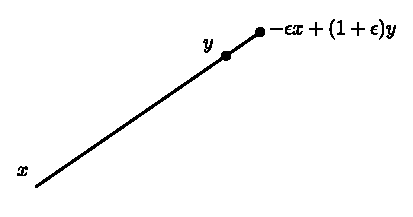
\includegraphics{figure/fig1.eps}
\end{figure}
\end{enumerate}
\end{definition}

In otherwords the line segment jointing $x$ and $y$ can be prolonged a little in $A$.

Clearly the empty set and any set consisting of one point are open convex sets. So open convex sets in $V$ need not necessarily be open in the topology of $V$.

Clearly the intersection of finitely many open convex sets is again an open convex set.

\begin{definition}\label{chap1-defi1.3.2}
Let $\{x_{1},\ldots,x_{n}\}\subset V$.
\end{definition}

An\pageoriginale {\em open convex combination} of $\{x_{1},\ldots,x_{n}\}$ is a convex combination $r_{1}x_{1}+\cdots+r_{n}x_{n}$ such that every coefficient $r_{i}>0$. The set of all points represented by such open convex combinations is denoted by $0(x_{1},\ldots,x_{n})$.

It is easily seen that $0(x_{1},\ldots,x_{n})$ is an open convex set. 

\begin{definition}\label{chap1-defi1.3.3}
If $\{x_{0},\ldots,x_{k}\}$ is independent, then $0(x_{0},\ldots,x_{k})$ is\break called an open $k$-simplex with vertices $\{x_{0},\ldots,x_{k}\}$. The number $k$ is called the dimension of the simplex $0(x_{0},\ldots,x_{k})$. If $\{i_{0},\ldots,i_{s}\}\subset\break \{0,\ldots,n\}$, then the open simplex $0(x_{i_{0}},\ldots,x_{i_{s}})$ is called a {\em $s$-face} (or a face) of $0(x_{0},\ldots,x_{k})$. If $s<k$, then, it is called a {\em proper face}.
\end{definition}

Clearly, the closed simplex $[x_{0},\ldots,x_{k}]$ is the disjoint union of $0(x_{0},\break\ldots,x_{k})$ and all its proper faces.

We give another class of examples of open convex sets below which will be used to construct other types of open convex sets.

\begin{definition}\label{chap1-defi1.3.4}
A {\em linear manifold} in $V$ is a subset $M$ of $V$ such that whenever $x$, $y\in M$ and $r\in\mathbb{R}$ then $rx+(1-r)y\in M$.
\end{definition}

Linear manifolds in $V$ are precisely the translates of subspaces of $V$; that is, if $V'$ is a subspace of $V$, and $z\in V$, then the set $z+V'=\{z+z'|z'\in V'\}$ is a linear manifold in $V$, and every linear manifold in $V$ is of this form. Moreover, given a linear manifold $M$ the subspace $V_{M}$ of $V$ of which $M$ is a translate is unique, namely,
$$
V_{M}=\{z-y|z\in M, y\in M\}=\{z-z'|z\in M,z'\text{~ a fixed element of~ } M\}. 
$$\pageoriginale

Thus the {\em dimension} of a linear manifold can be easily defined, and is equal to one less than the cardinality of any maximal independent subset of $M$ (see \ref{chap1-ex1.2.5}). A linear manifold of dimension 1, we will call a {\em line}. If $L$ is a line, $a$, $b\in L$, $a\neq b$, then every other point on $L$ is of the form $ta+(1-t)b$, $t\in \mathbb{R}$. If $M$ is a linear manifold in $V$ and $\dim M=(\dim V-1)$, then we call $M$ a {\em hyperplane} in $V$.

\begin{definition}\label{chap1-defi1.3.5}
Let $V$ and $W$ be real vector spaces. A function $\varphi:V\to W$ is said to be a linear map, if for every $t\in \mathbb{R}$ and every $x$, $y\in V$,
$$
\varphi(tx+(1-t)y)=t\varphi(x)+(1-t)\varphi(y).
$$
\end{definition}

Alternatively, one can characterize a linear map as being the sum of a vector space homomorphism and a constant.

\begin{ex}\label{chap1-ex1.3.6}
In definition \ref{chap1-defi1.3.5}, it is enough to assume the $\varphi(tx+(1-t)y)=t\varphi(x)+(1-t)\varphi(y)$ for $0\leq t\leq 1$.
\end{ex}

If $A$ is a convex set in $V$ and $\varphi:A\to W$, ($W$ a real vector space) is a map such that, for $x$, $y\in A$, $0\leq t\leq 1$
$$
\varphi(tx+(1-t)y)=t\varphi(x)+(1-t)\varphi(y),
$$
then also we call $\varphi$ {\em linear}. It is easy to see that $\varphi$ is the restriction to $A$ of a linear map of $V$ (which is uniquely defined on the linear manifold spanned by $A$). 

\begin{ex}\label{chap1-ex1.3.7}
Let $A$, $V$, $W$ be as above and $\varphi:A\to W$ a map. Show that $\varphi$ is linear if and only if the graph of $\varphi$ is convex. (graph of $\varphi$ is the subset of $V\times W$ consisting of $(x,y)$, $x\in A$, $y=\varphi(x)$). 
\end{ex}

\begin{ex}\label{chap1-ex1.3.8}
The\pageoriginale images and preimages of convex sets under a linear map (resp.\@ open convex sets) are convex sets (resp.\@ open convex sets). The images and preimages of linear manifolds under a linear map are again linear manifolds.
\end{ex}

A hyperplane $P$ in $V$ for instance is the preimage of $0$ under a linear map from $V$ to $\mathbb{R}$. Thus with respect to some basis of $V$, $P$ is given by an equation of the form $\sum \ell_{i}x_{i}=d$, where $x_{i}$ are co-ordinates with respect to a basis of $V$ and $\ell_{i}$, $d\in \mathbb{R}$  not all the $\ell_{i}$'s being zero. Hence $V-P$ consists of two connected components ($\sum \ell_{i}x_{i}>d$ and $\sum \ell_{i}x_{i}<d$), which we will call the {\em half-spaces} of $V$ determined by $P$. A half space of $V$ is another example of an open convex set.

\begin{definition}\label{chap1-defi1.3.9}
A {\em bisection} of a vector space $V$ consists of a triple $(P;H^{+},H^{-})$ consisting of a hyperplane $P$ in $V$ and the two half spaces $H^{+}$ and $H^{-}$ determined by $P$.
\end{definition}

These will be used in the next few section. A few more remarks: Let the dimension of $V=m$ and $V'$ be a $(m-k)$-dimensional subspace of $V$. Then extending a basis of $V'$ to a basis of $V$ we can express $V'$ as the intersection of $(k-1)$ subspace of $V$ of dimension $(m-1)$. Thus any linear manifold can be expressed as the intersection of finite set (non unique) of hyperplanes. Also we can talk of hyperplanes, linear submanifolds etc.\@ of a linear manifold $M$ in $V$. These could for example be taken as the translates of such from the corresponding subspace of $V$ or we can consider them as intersections of hyperplanes and linear manifolds in $V$\pageoriginale with $M$. Both are equivalent. Next, the topology on $V$ is taken to be topology induced by any Euclidean metric on $V$. The topology on subspaces of $V$ 
inherited from $V$ is the same as the unique topology defined by Euclidean metric on $V$. The topology on subspaces of $V$ inherited from $V$ is the same as the unique topology defined by Euclidean metrics on them. And for a linear manifold $M$ we can either take the topology on $M$ induced from $V$ or from subspace of $V$ of which it is a translate. Again both are the same. We will use these hereafter without more ado.

\section{The calculus of boundaries}\label{chap1-sec1.4}

\begin{definition}\label{chap1-defi1.4.1}
Let $A$ be an open convex set in $V$. A point $x\in V-A$ is called a {\em boundary point} of $A$, if there exists a point $a\in A$ such that $O(x,a)\in A$. The set of all boundary points of $A$ is called the {\em boundary} of $A$ and is denoted by $\partial A$. 
\end{definition}

A number of propositions will now be presented as exercises, and sometimes hints are given in the form of diagrams. In each given context a real vector space is involved even when it is not explicitly mentioned, and the sets we are considering are understood to be subsets of that vector space.

\begin{ex}\label{chap1-ex1.4.2}
A linear manifold has empty boundary. Conversely, if an open convex set $A$ has empty boundary, then $A$ is a linear manifold.
\end{ex}

\begin{remark*}
This uses the completeness of real numbers.
\end{remark*}

\begin{ex}\label{chap1-ex1.4.3}
If $(P;H^{+},H^{-})$ is a bisection of $V$, then $\partial H^{+}=\partial H^{-}=P$ and $\partial P=\emptyset$.
\end{ex}

\begin{proposition}\label{chap1-prop1.4.4}
If $A$ is an open convex set and $x\in \partial A$, then for all $b\in A$, $0(x,b)\subset A$.
\end{proposition}

\begin{proof}
Based\pageoriginale on this picture: There is `$a$' such that $0(x,a)\subset A$. Extend $a$, $b$ to a point $c\in A$. For any $q\in 0(x,b)$, there exists a $p\in 0(x,a)$ such that $q\in 0(c,p)$. Since $c$, $p\in A$, $q\in A$. Hence $0(x,b)\subset A$.
\begin{figure}[H]
\centering
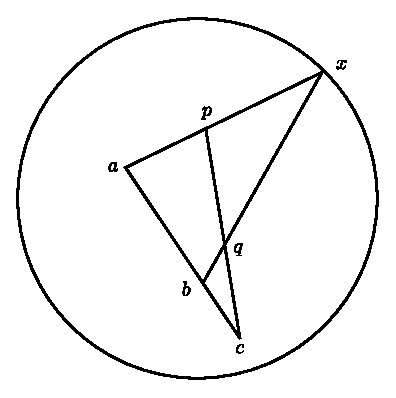
\includegraphics{figure/fig2.eps}
\end{figure}
\end{proof}

\begin{ex}\label{chap1-ex1.4.5}
Let $\varphi:V\to W$ be a linear map, and let $B$ be an open convex set in $W$. Then $\partial (\varphi^{-1}(B))(\varphi^{-1}(\partial B))$. If $\varphi$ is onto then equality holds.
\end{ex}

\begin{definition}\label{chap1-defi1.4.6}
The {\em closure} of an open convex set $A$ is defined to be $A\cup \partial A$; it is denoted by $\overline{A}$.
\end{definition}

\begin{ex}\label{chap1-ex1.4.7}
If $A\subset B$, then $\overline{A}\subset \overline{B}$.
\end{ex}

\begin{proposition}\label{chap1-prop1.4.8}
If $a$, $b\in A$ and $a\neq b$, where $A$ is an open convex set, then there is at most one $x\in \partial A$ such that $b\in 0(a,x)$.
\end{proposition}

\begin{proof}
If $b\in 0(a,x)$ and $b\in 0(a,y)$; $x$, $y\in \partial A$, $x\neq y$, then $0(a,x)$ and $0(a,y)$ lie on the same line, the line through $a$ and $b$ and both, are on the same side of $a$ as $b$. Either $x$ or $y$ must be closer to $a$ i.e.\@ either $x\in 0(a,y)$ or $y\in 0(a,x)$. If $x\in 0(a,y)$, then $x\in A$, but $A\cap \partial A=\emptyset$. Similarly $y\in 0(a,x)$ is also impossible. 
\end{proof}

\begin{proposition}\label{chap1-prop1.4.9}
Let $\{x_{0},\ldots,x_{n}\}$ be an independent set whose convex hull is contained in $\p A$, where $A$ is an open convex set. Let $a\in A$. Then $\{x_{0},\ldots,x_{n},a\}$ is independent.
\end{proposition}

\begin{proof}
\ref{chap1-prop1.4.8}\pageoriginale shows that each point of $K\{x_{0},\ldots,x_{n},a\}$ can be written as a unique convex combination. Hence by \ref{chap1-prop1.2.6} $\{x_{0},\ldots,x_{n},a\}$ is independent.
\end{proof}

\begin{proposition}\label{chap1-prop1.4.10}
Let $A$ and $B$ be open convex sets. If $B\subset \partial A$, then $\p B\subset \p A$.
\end{proposition}

\begin{proof}
Based on this picture:
\begin{figure}[H]
\centering
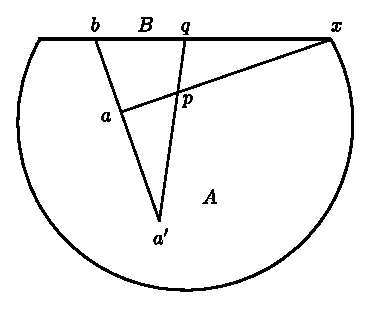
\includegraphics{figure/fig3.eps}
\end{figure}

The case $A$ or $B$ is empty is trivial. Otherwise, let $x\in \p B$, $b\in B$, $a\in A$; extend the segment $[b,a]$ to $a'\in A$. Let $p\in 0(x,a)$; then $q\in 0(x,b)$ can be found such that $p\in 0(q,a')$. Since $q\in 0(x,b)\subset B\subset \p A$, it follows that $0(q,a')\subset A$, therefore $p\in A$. Hence $0(x,a)\subset A$; obviously $x$ does not belong to $A$ and so $x\in \p A$.
\end{proof}

\begin{definition}\label{chap1-defi1.4.11}
If $A$ and $B$ are open convex sets, define $A<B$ to mean $A\subset \p B$.
\end{definition}

\ref{chap1-prop1.4.10} implies that $<$ is transitive.

\begin{ex}\label{chap1-ex1.4.12}
If $A$ is an open convex set, then $\overline{A}$ is convex.
\end{ex}

\noindent
{\bf Hint:}
\begin{figure}[H]
\centering
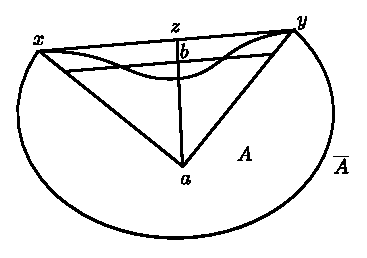
\includegraphics{figure/fig4.eps}
\end{figure}
\hfill$\Box$

\begin{proposition}\label{chap1-prop1.4.13}
If\pageoriginale $A$ and $B$ are open convex sets with $A\cap B\neq \emptyset$, then $\p(A\cap B)$ is the disjoint union of $\p A\cap B$, $A\cap \p B$ and $\p A\cap \p B$.
\end{proposition}

\begin{proof}
These three sets are disjoint, since $A\cap \p A=B\cap \p B\neq \emptyset$. Let $\mathscr{C} \in A \cap B$ and $x\in \p(A\cap B)$; since $x\in V-(A\cap B)=(V-A)\cup (V-B)$, $x$ either (1) belongs to $V-A$ and to $V-B$ or (2) belongs to $V-A$ and to $B$ or (3) belongs to $A$ and to $V-B$. Since $0(x,c)\subset A\cap B$, in case (1) $x\in \p A\cap \p B$, in case (2) $x\in \p A\cap B$ and in case (3) $x\in A\cap \p B$. The converse is similarly easy. 
\end{proof}

Another way of stating \ref{chap1-prop1.4.13} is to say that $\overline{A}\cap \overline{B}=\overline{A\cap B}$, when $A\cap B\neq \emptyset$.

\begin{proposition}\label{chap1-prop1.4.14}
If $A$ and $B$ are open convex sets and $A\subset \overline{B}$ and $A\cap B\neq \emptyset$, then $A\subset B$.
\end{proposition}

\begin{proof}
Let $c\in A\cap B$, and $a\in A$. The line from `$c$' to `$a$' may be prolonged a little bit to $a'\in A$. Since $a'\in \overline{B}$, it follows that $0(a',c)\subset B$, but $a\in 0(a',c)$. Hence $A\subset B$.
\end{proof}

\begin{proposition}\label{chap1-prop1.4.15}
If $\overline{A}=\overline{B}$, where $A$ and $B$ are open convex sets, then $A=B$. 
\end{proposition}

\begin{proof}
If $A\cap B=\emptyset$, since $A\cup \p A=B\cup \p B$, we have $A\subset \p B$ and $B\subset \p A$. By \ref{chap1-prop1.4.10} we have $A\subset \p A$ and $B\subset \p B$. But $A\cap \p A=\emptyset =B\cap\p B$. Hence $A\cap B=\emptyset$ is impossible except for the empty case. Then by  \ref{chap1-prop1.4.14}, $A\subset B$ and $B\subset A$. Therefore $A=B$.
\end{proof}

\begin{proposition}\label{chap1-prop1.4.16}
Let \; $\overline{0}(x_{1},\ldots,x_{n})$ denote the closure of
$0(x_{1},\ldots,\break x_{n})$. Then $\overline{0}(x_{1},\ldots,x_{n})=K\{x_{1},\ldots,x_{n}\}$. 
\end{proposition}

\begin{proof}
First,\pageoriginale $K\{x_{1},\ldots,x_{n}\}\subset\overline{0}(x_{1},\ldots,x_{n})$. For let $y\in K\{x_{1},\ldots,x_{n}\}$; then $y$ is a convex linear combination $r_{1}x_{1}+\cdots+r_{n}x_{n}$. Let $z=\dfrac{1}{n}(x_{1}+\cdots+x_{n})\in 0(x_{1},\ldots,x_{n})$. Then every point on the line segment $0(y,z)$ is obviously expressed as an open convex combination of $x_{1},\ldots,x_{n}$; hence $0(y,z)\subset 0(x_{1},\ldots,x_{n})$, and so $y\in \overline{0}(x_{1},\ldots,x_{n})$. 

Conversely, let $y\in \overline{0}(x_{1},\ldots,x_{n})$. If $y\in 0(x_{1},\ldots,x_{n})$, clearly $y\in K\{x_{1},\ldots,x_{n}\}$. Suppose $y\in \p 0(x_{1},\ldots,x_{n})$; let $z=\dfrac{1}{n}(x_{1}+\cdots+x_{n})$ as above. On the line segment $0(y,z)$, pick a sequence $a_{i}$ of points tending to $y$. Now, $a_{i}\in 0(y,z)\subset 0(x_{1},\ldots,x_{n})\subset K\{x_{i},\ldots,x_{n}\}$. Let $a_{i}=r_{i_{1}}x_{1}+\cdots+r_{i_{n}}x_{n}$. $r_{i_{j}}$ are bounded by $1$. By going to subsequences if necessary we can assume that the sequences $\{r_{i_{j}}\}$ converge for all $j$, say to $r_{j}$. Then $\sum r_{j}=1$, $r_{j}\geq 0$, and $\sum r_{i_{j}}x_{j}$ converge to $\sum r_{j}x_{j}\in K\{x_{1},\ldots, x_{n}\}$. But $\sum r_{i_{j}}x_{j}$ also converge to $y$. Hence $y=\sum r_{j}x_{j}$ and $y\in K\{x_{1},\ldots,x_{n}\}$.
\end{proof}

\begin{definition}\label{chap1-defi1.4.17}
An open convex set $A$ is said to be bounded, if for every line $L$ in $V$, there are points $x$, $y\in L$, such that $A\cap L\subset [x,y]$.
\end{definition}

Since in any case $A\cap L$ is an open convex set, either $A\cap L$ is empty, or $A\cap L$ consists of a single point, or $A\cap L$ is an open interval, possibly infinite on $L$. The boundedness of $A$ then implies that if $A\cap L$ contains at least two points, there are\pageoriginale $x$, $y\in L$ such that $A\cap L=0(x,y)$.

\begin{proposition}\label{chap1-prop1.4.18}
If $A$ is a bounded open convex set containing at least two points, then $\overline{A}=K(\p A)$.
\end{proposition}

\begin{proof}
Since $\p A\subset \overline{A}$ and $\overline{A}$ is convex, it is always true that $K(\p A)\subset \overline{A}$. Clearly $\p A\subset K(\p A)$. It remains only to show that $A\subset K(\p A)$. Let $a\in A$. Let $L$ be aline through `$a$' and another point $b\in A$ (such another point exists by hypothesis). Since $A$ is bounded, and $\{a,b\}\in L\cap A$, it follows that $A\cap L=0(x,y)$ for some $x$, $y\in L$. Clearly $x$, $y\in \p A$, and $a\in [x,y]\subset K(\p A)$.
\end{proof}

\begin{remark*}
With the hypothesis of \ref{chap1-prop1.4.18}, we have $\overline{A}=\bigcup\limits_{y}[a,y]$, `$a$' a fixed point of $A$ and $y\in \p A$ and $A=\bigcup\limits_{y}0(a,y)\cup \{a\}$. 
\end{remark*}

\begin{ex}\label{chap1-ex1.4.19}
If $A$ and $B$ are open convex sets, and $A<B$, and $B$ is bounded, then $A$ is bounded.
\end{ex}

\noindent
{\bf Hint:}
\begin{figure}[H]
\centering
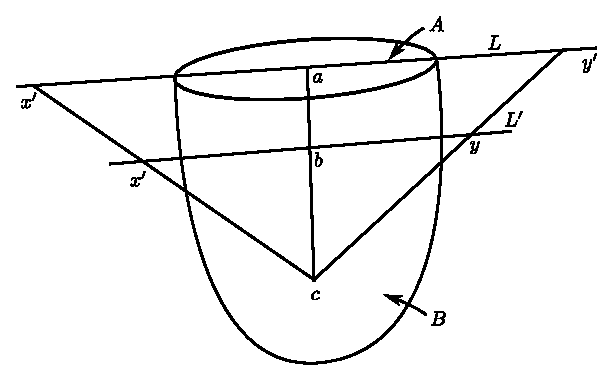
\includegraphics{figure/fig5.eps}
\end{figure}
\hfill$\Box$

\begin{ex}\label{chap1-ex1.4.20}
Let\pageoriginale $A$ be an open convex set in $V$, and $B$ be an open convex set in $W$. Then (1) $A\times B$ is an open convex set in $V\times W$; (2) $\p (A\times B)$ is the disjoint union of $\p A\times B$, $A\times \p B$ and $\p A\times \p B$; (3) $A\times B$ is bounded if and only if $A$ and $B$ are, provided $A\neq \emptyset$, $B\neq \emptyset$.
\end{ex}

The following two exercises are some what difficult in the sense they use compactness of the sphere, continuity of certain functions etc.

\begin{ex}\label{chap1-ex1.4.21}
The closure of $A$ defined above (\ref{chap1-defi1.4.6}) coincides with the topological closure of $A$ in $V$.
\end{ex}

\begin{ex}\label{chap1-ex1.4.22}
An open convex set which is bounded in the sense of some Euclidean metrix is bounded in the above sense, and conversely.
\end{ex}

\section{Convex cells}\label{chap1-sec1.5}

\begin{definition}\label{chap1-defi1.5.1}
An {\em open convex cell} is defined to be a finite intersection of hyperplanes and half spaces, which as an open convex set is bounded.
\end{definition}

Clearly the intersection of two open convex cells is an open convex cell, and the product of two open convex cells is an open convex cell.

With respect to a coordinate system in the vector space in which it is defined, an open convex cell is given by a finite system of linear inequalities. If $A$ is an open convex cell, by taking the intersection of all the hyperplanes used in defining $A$, we can write $A=P\cap H_{1}\cap \ldots\cap H_{\ell}$, where $P$ is a linear manifold and\pageoriginale $H_{i}$ are half spaces. Since $H_{i}$ are open in the ambient vector space $A$ is open in $P$. Let $A=P'\cap H_{1}'\cap\ldots\cap H_{\ell'}'$ be another such representation of $A$. If $A$ is nonempty, then $P=P'$. For $A\subset P\cap P'$
and if $P\neq P'$, $P\cap P'$ is of lower dimension than $P$, hence $A$ cannot be open in $P$. Thus $P'=P$; though the $H_{i}$'s and $H'_{j}$'s may differ. Hence $P$ can be described as the unique linear manifold which contains $A$ as an open subset. We define the {\em dimension} of the open convex cell $A$ to be the dimension of the above linear manifold $P$. If $A=\emptyset$, we define the dimension of $A$ to be $-1$.

If $A$ is an open convex cell, we will call $\overline{A}$ a {\em closed convex cell}. The {\em boundary} of a closed convex cell is defined to be the same as the boundary of the open convex cell of which it is the closure. This is well defined, since $\overline{A}=\overline{B}$ implies $A=B$, when $A$ and $B$ are open convex sets (\ref{chap1-prop1.4.15}). The {\em dimension} of $\overline{A}$ is defined to be the same as the dimension of $A$.

Using \ref{chap1-prop1.2.9} and \ref{chap1-ex1.2.10}, it is easily seen that the dimension of $A$ is one less than the cardinality of maximal independent set contained in $A$ or $\overline{A}$. Similar remark applies for $\overline{A}$ also. Actually, using this description we can extend the definition of dimension to arbitrary convex sets.

\begin{ex}\label{chap1-ex1.5.2}
If $A$ is an open convex cell of dimension $K$, and $A_{1},\ldots,A_{n}$ are open convex cells of dimension $<K$, then $A\not\subset A_{1}\cup \ldots \cup A_{n}$. 
\end{ex}

\begin{proposition}\label{chap1-prop1.5.3}
An open $k$-simplex is an open convex cell of dimension $k$. A closed $k$-simplex is a closed convex cell of dimension\pageoriginale $k$.
\end{proposition}

\begin{proof}
It is enough to prove for the open $k$-simplex. Let the open $k$-simplex be $0(x_{0},\ldots,x_{k})=A$ in the vector space $V$. The the unique linear manifold $P$ containing $A$ is the set of points $r_{0}x_{0}+\cdots+r_{k}x_{k}$, where $r_{0}+\cdots+r_{k}=1$, $r_{i}\in \mathbb{R}$. Define $\varphi_{i}(r_{0}x_{0}+\cdots+r_{k}x_{k})=r_{i}$; $\varphi_{i}$ is a linear map from $P$ to $\mathbb{R}$. Then $H_{i}=\varphi^{-1}_{i}(0,\infty)$ is a half space relative to the hyperplane $P$ and $0(x_{0},\ldots,x_{k})=H_{0}\cap \ldots\cap H_{k}$. By extending $H_{i}$ to half spaces $H'_{i}$ in $V$ suitably, $0(x_{0},\ldots,x_{k})=P\cap H'_{0}\cap \ldots\cap H'_{k}$. Boundedness of $A$,   and that $\dim A=k$ are clear.
\end{proof}

\begin{proposition}\label{chap1-prop1.5.4}
Let $A$ be a nonempty open cell. Then there is a finite set $\mathscr{P}=\{A_{1},\ldots,A_{k}\}$ whose elements are open convex cells, such that
\begin{itemize}
\item[\rm(a)] $\overline{A}=\bigcup\limits_{1\leq i\leq k}A_{i}$.

\item[\rm(b)] $A_{i}\cap A_{j}=\emptyset$ if $i\neq j$

\item[\rm(c)] $A$ is one of the cells $A_{i}$

\item[\rm(d)] The boundary of each element of $\mathscr{P}$ is union of elements of $\mathscr{P}$. (Of course the empty set is also taken as such a union). 
\end{itemize}
\end{proposition}

\begin{proof}
Let $A=P\cap H_{1}\cap \ldots\cap H_{n}$, where $P$ is a linear manifold and $H_{i}$ are half spaces with boundary hyperplanes $P_{i}$. Let $\mathscr{P}$ be the set whose elements are nonempty sets of the following sort:

Let
$$
\{1,\ldots,n\}=\{j_{1},\ldots,j_{q}\}\cup \{k_{1},\ldots,k_{n-q}\}.
$$

Then if it is not empty the set $P\cap H_{j_{1}}\cap\ldots\cap H_{j_{q}}\cap P_{k_{1}}\cap\ldots\cap P_{k_{(n-q)}}$ is\pageoriginale an element of $P$. The properties of $\mathscr{P}$ follow from \ref{chap1-prop1.4.13}.

If the above, the union of elements of $\mathscr{P}$ excluding $A$ constitute the boundary $\p A$ of $A$. Then using \ref{chap1-prop1.4.9}, and the remarks preceding \ref{chap1-ex1.5.2}, we have, if $A_{i}\in \mathscr{P}$, $A_{i}\neq A$, then $\dim A_{i}<\dim A$. We have seen that if $A$ is a bounded open convex set of $\dim \geq 1$, then $\overline{A}=K(\p A)$. Hence by an obvious induction, we have 
\end{proof}

\begin{proposition}\label{chap1-prop1.5.5}
A closed convex cell is the convex hull of a finite set of points.
\end{proposition}

A partial converse of \ref{chap1-prop1.5.5}, is trivial:

\setcounter{subsection}{5}
\subsection{}\label{chap1-sec1.5.6}
The convex hull of a finite set is a finite union of open (closed) convex cells.

The converse of \ref{chap1-prop1.5.5} is also true.

\setcounter{proposition}{6}
\begin{ex}\label{chap1-ex1.5.7}
The convex hull of a finite set is a closed convex cell.
\end{ex}

\noindent
{\bf Hint:} Let $\{x_{1},\ldots,x_{n}\}$ be a finite set in vector space $V$. By 
\ref{chap1-prop1.4.16} $K\{x_{1},\ldots,x_{n}\}=\overline{0}(x_{1},\ldots,x_{n})$. It is enough to show that $0(x_{1},\ldots,x_{n})$ is an open convex cell. Let $M$ be the linear manifold generated by $\{x_{1},\ldots,x_{n}\}$. Let $\dim M=k$. Write $A=0(x_{1},\ldots,x_{n})$, $\overline{A}=K\{x_{1},\ldots,x_{n}\}$. $A$ is open in $M$. To prove the proposition it is enough to show that $A$ is the inter section of half spaces in $M$.

\begin{step}\label{chap1-step1}
$\overline{A}$ and $\p A$ are both union of open (hence closed) simplexes with vertices in $\{x_{1},\ldots,x_{n}\}$. The assertion for $\overline{A}$ follows from \ref{chap1-prop1.2.7}.
\end{step}

\begin{step}%2
If\pageoriginale $B$ is a $(k-1)$-simplex in $\p A$ and $N$ is the hyperplane in $M$ defined by $B$, then $A$ cannot have points in both the half spaces defined by $N$ in $M$.
\end{step}

\begin{step}%3
It is enough to show that each point of $\p A$ belongs to a closed $(k-1)$-simplex with vertices in $\{x_{1},\ldots,x_{n}\}$.
\end{step}

\begin{step}%4
Each point $x\in \p A$ is contained in a closed $(k-1)$-simplex with verticer in $\{x_{1},\ldots,x_{n}\}$. To prove this let $C_{1},\ldots,C_{p}$ be the closed simplexes contained in $\p A$ with vertices in $x_{1},\ldots,x_{n}$ which contain $x$, and $D_{1},\ldots,D_{q}(\subset\p A)$ which do not contain $x$. By Step (1) $\bigcup\limits_{i}C_{i}\bigcup\limits_{j}D_{j}=\p A$. Consider any point $a\in A$ and a point $b\in 0(a,x)$. Let $C'_{i}$ (resp.\@ $D'_{j}$) denote the closed simplex whose vertices are those of $C_{i}$ (resp.\@ $D_{j}$) and `$a$'. By the remark following \ref{chap1-prop1.4.18}. $\bigcup\limits_{i}C'_{i}\bigcup\limits_{j}D'_{j}=\overline{A}$. Show that $\bigcup\limits_{i}C_{i}'$ is a neighbourhood of $b$. If $\dim C_{i}<k-1$ for all $i$, then $\dim C'_{i}\leq k-1$ for all $i$. Use \ref{chap1-ex1.5.2} to show that in this case $\bigcup C'_{i}$ cannot be a neighbourhood of $b$.
\end{step}

Since the linear image of convex hull of a finite set is also the convex hull of finite set, \ref{chap1-ex1.5.7}, immediately gives that the linear image of a closed convex cell is a closed convex cell. If $A$ is an open convex cell in $V$ and $\varphi$ a linear map from $V$ to $W$, then $\varphi(\overline{A})=\overline{\varphi(A)}$, by \ref{chap1-prop1.4.16}, hence by \ref{chap1-prop1.4.15} $\varphi(A)$ is an open convex cell. Therefore

\begin{proposition}\label{chap1-prop1.5.8}
The linear image of an open (resp.\@ closed) convex cell is an open (resp.\@ closed) convex cell.
\end{proposition}

\section{Presentations of polyhedra}\pageoriginale\label{chap1-sec1.6}

If $\mathscr{P}$ is a set of sets and $A$ is set, we shall write
$$
A\vee \mathscr{P}
$$
when $A$ is a union of elements of $\mathscr{P}$. For example (d) of \ref{chap1-prop1.5.4} can be expressed as ``If $A\in \mathscr{P}$, then $\p A\vee \mathscr{P}$''. We make the obvious convention, when $\emptyset$ is the empty set, that $\phi\vee \mathscr{P}$ no matter what $\mathscr{P}$ is.

\begin{definition}\label{chap1-defi1.6.1}
A {\em polyhedral presentation} is a finite set $\mathscr{P}$ whose elements are open convex cells, such that $A\in \mathscr{P}$ implies $\p A\vee \mathscr{P}$. 
\end{definition}

\begin{definition}\label{chap1-defi1.6.2}
A {\em regular presentation} is a polyhedral presentation $\mathscr{P}$ such that any two distinct elements are disjoint, that is, $A\in\mathscr{P}$, $B\in\mathscr{P}$, $A\neq B$ implies $A\cap B=\emptyset$.
\end{definition}

\begin{ex*}
The $\mathscr{P}$ of proposition \ref{chap1-prop1.5.4} is a regular presentation. 
\end{ex*}

\begin{definition}\label{chap1-defi1.6.3}
A {\em simplicial presentation} is a regular presentation\break whose elements are simplicies and such that if $A\in \mathscr{P}$, then every fact of $A$ also belongs to $\mathscr{P}$.
\end{definition}

If $\mathcal{Q}\subset \mathscr{P}$ are polyhedral presentations, we call $\mathcal{Q}$ a {\em subpresentation} of $\mathscr{P}$. If $\mathscr{P}$ is regular (resp.\@ simplicial) then $\mathcal{Q}$ is necessarily regular (resp.\@ simplicial). The points of the $O$-cells of a simplicial presentation will be called the {\em vertices} of the simplicial presentation. The {\em dimension} of a polyhedral presentation $\mathscr{P}$ is defined to be the maximum of the dimensions of the open cells of $\mathscr{P}$.

\begin{definition}\label{chap1-defi1.6.4}
If $\mathscr{P}$ is a polyhedral presentation $|\mathscr{P}|$ will be\pageoriginale used to denote the union of all elements of $\mathscr{P}$. We say that $\mathscr{P}$ {\em is a presentation} of $|\mathscr{P}|$ or that $|\mathscr{P}|$ {\em has a presentation} $\mathscr{P}$.
\end{definition}

Recall that in \ref{chap1-sec1.1}, we have defined a polyhedron as a subset of a real vector space, which is a finite union of convex hulls of finite sets. It is clear consequence of \ref{chap1-prop1.5.4}, \ref{chap1-prop1.5.5} and 
\ref{chap1-sec1.5.6} that

\begin{proposition}\label{chap1-prop1.6.5}
Every polyhedron has a polyhedral presentation. If $\mathscr{P}$ is a polyhedral presentation, then $|\mathscr{P}|$ is a polyhedron.
\end{proposition}

Thus, if we define a polyhedron as a subset of a real vector space which has a polyhedral presentation, then this definition coincides with the earlier definition. 

\begin{proposition}\label{chap1-prop1.6.6}
The union or intersection of a finite number of polyhedra is again a polyhedron. 
\end{proposition}

\begin{proof}
It is enough to prove for two polyhedra say $P$ and $Q$. Let $\mathscr{P}$ and $\mathcal{Q}$ be polyhedral presentations of $P$ and $Q$ respectively. Then $\mathscr{P}\cup \mathcal{Q}$ is a polyhedral presentation of $P\cup Q$; hence $P\cup Q$ is a polyhedron. To prove that $P\cap Q$ is a polyhedron, consider the set $\mathscr{R}$ consisting of all nonempty sets of the form $A\cap B$, for $A\in \mathscr{P}$ and $B\in\mathcal{Q}$. It follows from \ref{chap1-prop1.4.13} that $\mathscr{R}$ is a polyhedral presentation. Clearly $|\mathscr{R}|=P\cap Q$. Hence by \ref{chap1-prop1.6.5} $P\cap Q$ is a polyhedron.
\end{proof}

If $X \subset Y$ are polyhedra, we will call $X$ a {\em subpolyhedron} of $Y$. Thus in \ref{chap1-prop1.6.6}, $P\cap Q$ is a subpolyhedron of both $P$ and $Q$. 

\setcounter{subsection}{6}
\subsection{}\label{chap1-sec1.6.7}
If $\mathscr{P}$ and $\mathcal{Q}$ are two polyhedral presentations consider the sets of the form $A\times B$, $A\in \mathscr{P}$, $B\in \mathcal{Q}$. Clearly $A\times B$ is an\pageoriginale open convex cell, and by \ref{chap1-ex1.4.20} $\p (A\times B)$ is the disjoint union of $\p A\times B$, $A\times \p B$ and $\p A\times \p B$. Thus the set of cells of the form $A\times B$, $A\in \mathscr{P}$, $B\in \mathcal{Q}$ is a polyhedral presentation, regular if both $\mathscr{P}$ and $\mathcal{Q}$ are. This we will denote by $\mathscr{P}\times \mathcal{Q}$. As above, we have, as a consequence that $P\times Q$ is a polyhedron, with presentation $\mathscr{P}\times \mathcal{Q}$.

\setcounter{proposition}{7}
\begin{ex}\label{chap1-ex1.6.8}
The linear image of a polyhedron is a polyhedron (follows from the definition of polyhedron and the definition of linear map).
\end{ex}

Recall that we have defined a polyhedral map between two polyhedra as a map whose graph is a polyhedron.

\begin{proposition}\label{chap1-prop1.6.9}
The composition of two polyhedral maps is a polyhedral map.
\end{proposition}

\begin{proof}
Let $X$, $Y$ and $Z$ be three polyhedra in the vector spaces $U$, $V$ and $W$ respectively, and let $f:X\to Y$, $g:Y\to Z$ be polyhedral maps. Then $\Gamma(f)\subset U\times V$ and $\Gamma(g)\subset V\times W$ are polyhedra. By \ref{chap1-sec1.6.7}, $\Gamma(f)\times Z$ and $X\times \Gamma(g)$ are also polyhedra in $U\times V\times W$. By \ref{chap1-prop1.6.6}, $(\Gamma(f)\times Z)\cap (X\times \Gamma(g))$ is a polyhedron. This intersection is the set
$$
S:\{(x,y,z)\mid x\in X,\ y=f(x),\ z=g(y)\}
$$
in $U\times V\times W$. By \ref{chap1-ex1.6.8} the projection of $U\times V\times W$ to $U\times W$ takes $S$ into a polyhedron, which is none other than the graph of the map $g\circ f:X\to Z$. Hence $g\circ f$ is polyhedral.
\end{proof}

If a polyhedral map $f:P\to Q$, is one-to-one and onto we term it a {\em polyhedral equivalence}.

\begin{ex}\label{chap1-ex1.6.10}
If, $f:P\to Q$ is a polyhedral map, then the map $g:P\to \Gamma(f)$\pageoriginale defined by $f'(x)=(x,f(x))$ is a polyhedral equivalence. 
\end{ex}

\setcounter{subsection}{10}
\subsection{Dimension of a polyhedron}\label{chap1-sec1.6.11}

~\phantom{a}

The dimension of a polyhedron $P$ is a defined to be Max.\@ $\dim \mathcal{C}$, $\mathcal{C}\in \mathscr{P}$, where $\mathscr{P}$ is any polyhedral presentation of $P$. 

OF course we have to check that this is independent of the presentation chosen. This follows from \ref{chap1-ex1.5.2}.

Let $P$ and $Q$ be two polyhedra and $f:P\to Q$ be a polyhedral map. Let $\gamma:P\times Q\to P$ and $\mu:P\times Q\to Q$ be the first and second projections. If $\mathscr{C}$ is any presentation of $\Gamma(f)$, then the open cells of the form $\lambda(C)$, $C\in \mathscr{C}$ is a presentation of $P$, regular if and only if $\mathscr{C}$ is regular. If $f$ is a polyhedral equivalence, then the cells of the form $\mu(C)$, $C\in\mathscr{C}$ is a presentation of $Q$. This shows that

\setcounter{proposition}{11}
\begin{proposition}\label{chap1-prop1.6.12}
The dimension of a polyhedron is a polyhedral invariant.
\end{proposition}

\section{Refinement by bisection}\label{chap1-sec1.7}

\begin{definition}\label{chap1-defi1.7.1}
If $\mathscr{P}$ and $\mathcal{Q}$ are polyhedral presentations, we say that $\mathscr{P}$ {\em refines} $\mathcal{Q}$, or $\mathscr{P}$ is a {\em refinement} of $\mathcal{Q}$ provided
\begin{itemize}
\item[(a)] $|\mathscr{P}|=|\mathcal{Q}|$

\item[(b)] If $A\in \mathscr{P}$, and $B\in \mathcal{Q}$, then $A\cap B=\emptyset$ or $A\subset B$.
\end{itemize}
\end{definition}

In otherwords, $\mathscr{P}$ and $\mathcal{Q}$ are presentations of the same polyhedron and each element (an open convex cell) of $\mathscr{P}$ is contained in each element of $\mathcal{Q}$ which it intersects. Hereafter, when there is\pageoriginale no confusion, we will refer to open convex cells and closed convex cells as {\em open cells} and {\em closed cells}. A polyhedral presentation is regular if and only if it refines itself.

Let $\mathscr{B}=(P;H^{+},H^{-})$ be a bisection of the ambient vector space $V$ 
(\ref{chap1-defi1.3.9}); $\mathfrak{a}$ a polyhedral presentation of a polyhedraon in $V$, and let $A\in \mathfrak{a}$. We say that {\em $\mathfrak{a}$ admits a bisection by $\mathscr{B}$ at $A$, provided:} 

Whenever an open cell $A_{1}\in \mathfrak{a}$ intersects $\p A$ (i.e.\@ $A_{1}\cap \p A\neq \emptyset$), and $\dim A_{1}<\dim A$, then either $A_{1}\subset P$ or $A_{1}\subset H^{+}$ or $A_{1}\subset H^{-}$ (in particular this should be true for any cell in the boundary of $A$).

If $\mathfrak{a}$ admits a bisection by $\mathscr{B}$ at $A$, then we define a presentation $\mathfrak{a}'$ as follows, and call it the {\em result of bisecting $\mathfrak{a}$ by $\mathscr{B}$ at $A$}:

$\mathfrak{a}'$ consists of $\mathfrak{a}$ with the element $A$ removed, and with the nonempty sets of the form, $A\cap P$ or $A\cap H^{+}$ or $A\cap H^{-}$, that is 
$$
\mathfrak{a}'=\Big\{(\mathfrak{a}-\{A\})\cup \{A\cap P, A\cap H^{+},\ A\cap H^{-}\}-\{\emptyset\}\Big\}.
$$

By \ref{chap1-prop1.4.13}, and the definition of admitting a bisection, $\mathfrak{a}'$ is a polyhedral presentation. Clearly $\mathfrak{a}'$ refines $\mathfrak{a}$, if $\mathfrak{a}$ is regular.

We remark that it may well be the case that $A$ is contained in $P$ or $H^{+}$ or $H^{-}$. In this event, bisecting at $A$ changes nothing at all, that is $\mathfrak{a}'=\mathfrak{a}$. If this is the case we call the bisection {\rm trivial}. It is also possible, in the case of irregular\pageoriginale presentations, that some or all of the sets $A\cap P$, $A\cap H^{+}$, $A\cap H^{-}$ may already be contained in $\mathfrak{a}-\{A\}$ in this event, bisection will not change as much as we might expect.

\begin{ex}\label{chap1-ex1.7.2}
Let $A$ and $B$ be two open cells, with $\dim A \leq \dim B$ and $A\neq B$. Let $\mathscr{B}_{j}:\{P_{j};H^{+}_{j},H^{-}_{j}\}_{1\leq j\leq m}$ be bisections of space such that $A$ is the intersection of precisely one element from some of the $\mathscr{B}_{j}$'s. If $A\cap B\neq \emptyset$, then $\exists$ an $\ell$, $1\leq \ell\leq m$, such that $B\cap P$, $B\cap H^{+}$ and $B\cap H^{-}$ are all nonvacuous.
\end{ex}

What we are aiming at is to show that every polyhedral presentation $\mathscr{P}$ has a regular refinement, which moreover is obtained from $\mathscr{P}$ by a particular process (bisections). The proof is by an obvious double induction; we sketch the proof below leaving some of the details to the reader.

\begin{proposition}\label{chap1-prop1.7.3}
REFI $(\mathscr{P},\mathscr{P}',\{S_{i}\})$

There is a procedure, which, applied to a polyhedral presentation $\mathscr{P}$, gives a finite sequences $\{S_{i}\}$ of bisections (at cells by bisections of space), which start on $\mathscr{P}$, give end result $\mathscr{P}'$, and $\mathscr{P}'$ is a regular presentation which refines $\mathscr{P}$. 
\end{proposition}

\begin{proof}
\setcounter{step}{0}
\begin{step}%%% 1
First, we find a finite set $\mathscr{B}_{j}:\{P_{j};H^{+}_{j},H^{-}_{j}\}$, $j=1,\ldots n$ of bisections of the ambient space, such that every element of $\mathscr{P}$ is an intersection one element each from some of the $\mathscr{B}_{j}$'s. This is possible because every element of $\mathscr{P}$ is a finite intersection of hyperplanes and half spaces, and there are only a finite number of elements in $\mathscr{P}$.  
\end{step}

\begin{step}%% 2
Write\pageoriginale $\mathscr{P}=\mathscr{P}_{0}$. Index the cells of $\mathscr{P}_{0}$ in such a way that the dimension is a non decreasing function. That is define $p_{0}$ to be the cardinality of $\mathscr{P}_{0}$, arrange the elements of $\mathscr{P}_{0}$ as $D^{0}_{0},\ldots,D^{0}_{p_{0}}$, such that $\dim D^{0}_{k}\leq \dim D^{0}_{k+1}$ for all $0\leq k\leq p_{0}-1$. 
\end{step}

\begin{step}%3
$S_{0,1}$ denotes the process of bisecting $\mathscr{P}_{0}$ at $D^{0}_{0}$ by $\mathscr{B}_{1}$. Inductively, we define $S_{0,k+1}$ to be the process of bisecting $\mathscr{P}_{0,k}$ at $D^{0}_{k+1}$ by $\mathscr{B}_{1}$; and $\mathscr{P}_{0,k+1}$ the result. This is well defined since the elements of $\mathscr{P}_{0}$ are arranged in the order of nondecreasing dimension. This can be done until we get $S_{0,p_{0}}$ and $\mathscr{P}_{0,p_{0}}$. 
\end{step}

\begin{step}%4
Write $\mathscr{P}_{1}=\mathscr{P}_{0,p_{0}}$, repeat step (2) and then the step (3) with bisection $\mathscr{B}_{2}$ instead of $\mathscr{B}_{1}$. 
\end{step}

And so on until we get $\mathscr{P}_{n}$, when the process stops. $\mathscr{P}_{n}$ is clearly a refinement of $\mathscr{P}=\mathscr{P}_{0}$; it remains to show that $\mathscr{P}_{n}$ is regular. Each element by $\mathscr{P}_{n}$ belongs to some $\mathscr{P}_{i,j}$ and each element of $\mathscr{P}_{n}$ is a finite intersection of exactly one element each from a subfamily of the $\mathscr{B}_{j}$'s. It is easily shown by double induction that if $A\in \mathscr{P}_{n}$, then for any $j$, $i\leq j\leq n$, either $A\subset P_{j}$ or $A\subset H^{+}_{j}$ or $A\subset H^{-}_{j}$. That is $\mathscr{P}_{n}$ admits a bisection at $A$ by $\mathscr{B}_{j}$ for any $j$, but the bisection is trivial. Let $C$, $D\in\mathscr{P}_{n}$, $C\neq D$ $C\cap  D\neq \emptyset$, $\dim C\leq \dim D$. Then since $C$ is an intersection of one element each from a subfamily of the $\mathscr{B}_{j}$'s, by 
\ref{chap1-prop1.7.3}, there exists an $\ell$ such that $D\cap P_{\ell}$, $D\cap H^{+}_{\ell}$ and $D\cap H^{-}_{\ell}$ are all nonempty. But this is a contradiction. Hence $\mathscr{P}_{n}$ is regular. Write $\mathscr{P}_{n}=\mathscr{P}'$,\pageoriginale $S_{i,j}=S_{p_{0}}+\cdots+p_{i}+j$. This gives the ``REFI $(\mathscr{P},\mathscr{P}',\{S_{i}\})$''.
\end{proof}

We can now draw a number of corollaries:

\begin{corollary}\label{chap1-coro1.10.4}
Any polyhedron has a regular presentation.
\end{corollary}

\begin{corollary}\label{chap1-coro1.10.5}
Any two polyhedral presentations $\mathscr{P}$, $\mathcal{Q}$ of the same polyhedron $X$ have a common refinement $\mathscr{R}$, which is obtained from $\mathscr{P}$ and from $\mathcal{Q}$ by a finite sequence of bisections.

To see this, note that $\mathscr{P}\cup \mathcal{Q}$ is a polyhedral presentation of $X$. The application REFI $(\mathscr{P}\cup \mathcal{Q},\mathscr{R},\{S_{i}\})$ provides $\mathscr{R}$. Let $\{T_{i}\}$ and $\{U_{k}\}$ denote the subsequences applying to $\mathscr{P}$ and $\mathcal{Q}$ respectively; observe that they both result in $\mathscr{R}$.
\end{corollary}


\begin{corollary}\label{chap1-coro1.10.6}
Given any finite number $\mathscr{P}_{1},\ldots,\mathscr{P}_{r}$ of polyhedral presentations, there is a regular presentation $\mathcal{Q}$ of $|\mathscr{P}_{1}|\cup\ldots\cup |\mathscr{P}_{r}|$, and $\mathcal{Q}$ has subpresentations $\mathcal{Q}_{1},\ldots,\mathcal{Q}_{r}$, with $|\mathscr{P}_{i}|=|\mathcal{Q}_{i}|$ for all $i$ and $\mathscr{P}_{i}$ is obtained from $\mathcal{Q}_{i}$ by a finite sequence of bisections.

This is an application of REFI $(\mathscr{P}_{1}\cup \ldots\cup \mathscr{P}_{r},\mathcal{Q},\{S_{i}\})$ and an analysis of the situation. 
\end{corollary}







